\section{Backtracking (Podas)}

	La descripción del problema como la forma de pensarlo son las mismas que el ejercicio anterior.

\subsection{Resolución}
	
	Además de lo dicho en el ejercicio anterior, la idea es podar más el árbol para no recorrer ramas donde no nos interese su solución o sea un caso inválido. Para esto tenemos 2 podas, la primera consiste en no ramas que no mejoren mi mejor solución hasta el momento y la segunda consiste en hacer un análisis a futuro de la confiabilidad de los agentes. Para la primera consideremos un conjunto con "k" elementos en el, "a" representa la cantidad total de agentes e "i" representa los agentes que ya fueron evaluados, la poda consiste en que si $k+(a-i)$ <= s (notar que "a-i" representa los agentes que faltan por evaluar), donde s es la mejor solución hasta el momento, si esto pasa no seguimos recorriendo esa rama ya que no aporta nada mejor a lo que tenemos. La otra consiste en hacer un mejor chequeo de la confiabilidad. Además de lo descripto en el ejercicio anterior, vemos que si el agente a ser agregado, llamemoslo "x", confia en otro agente "y", "y" pueda formar parte del conjunto.  Para esto vereficamos la confiabilidad de "y" si resulta que no podemos agregarlo al conjunto tampoco agregamos a "x" por lo que no recorremos esa posibilidad. 
	
\subsection{Pseudocódigo}  
	
\begin{algorithm}[H]
\caption{BacktrackingPodas}\label{Ej1.1}

\begin{algorithmic}[H]
\Procedure{BacktrackingPodas}{vector(pair(agente, agente)) encuestas, agentes, ConjAgentes}
\If{Si no me quedan agentes para evaluar}
\If{longitud(ConjAgentes) > solucion}
\State solucion $=$ longitud(ConjAgentes)
\EndIf
\EndIf
\If{PuedoAgregarAgente $\wedge$ PuedeSerMejorSolución}
\State Paso Recursivo rama agregueAlAgente
\EndIf
\If{PuedeSerMejorSolución}
\State Paso Recursivo rama NoAgregoAlAgente
\EndIf
\EndProcedure
\end{algorithmic}

\end{algorithm}

\subsection{Demostración de correctitud}
	
	En este caso podemos decir que esta demostración es muy similar a la hecha en el algoritmo anterior. Lo que agregamos son las podas al árbol, esto hace que cosideremos menos ramas. Lo que hay que ver ahora es que no estamos descartando ninguna solución válida. Pero como dijimos antes las podas sólo descartan soluciones inválidas (la diferencia con el algoritmo anterior es que la poda verifica validez a futuro y no sólo a presente) y soluciones que no mejoran la mejor solución hasta el momento. Al igual que antes descartamos soluciones en los nodos internos, en vez de descartarlas en las hojas y nos aseguramos de recorrer todas las otras soluciones.

\subsection{Complejidad}

	Dado que las podas no agregan complejidad al algoritmo ya que se aprovechan de lo que se hacía antes y en peor caso tengo que recorrer todo el árbol, la complejidad en peor caso sigue siendo lo misma que el ejercicio anterior. O($2^{i}*((i*a^{2})+(i^{2}*a))$). 
	
\subsection{Experimentación}

	Para experimentar consideramos las mismas instancias que el algoritmo anterior. Las instancias fueron generadas de la misma forma que en la sección anterior.	

\begin{figure}[h]
\begin{subfigure}{0.5\textwidth}
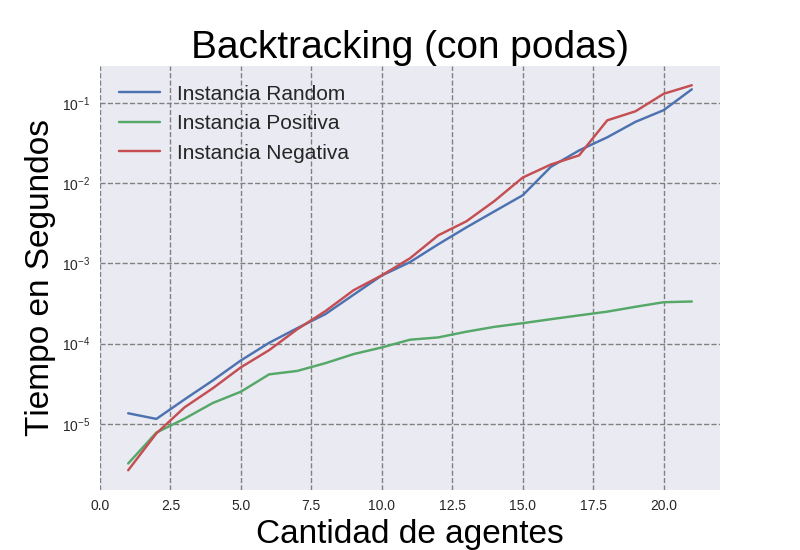
\includegraphics[scale=0.45]{BacktrackingPodasLog.png}
\end{subfigure}
\begin{subfigure}{0.5\textwidth}
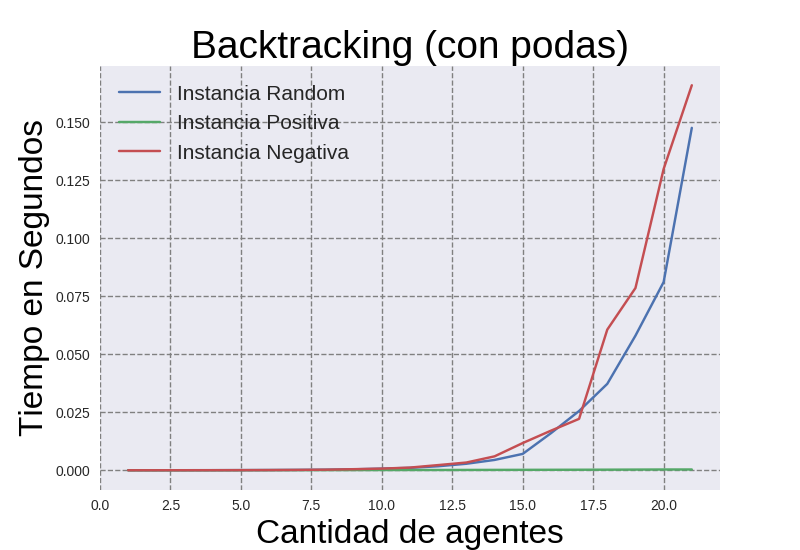
\includegraphics[scale=0.45]{BacktrackingPodas.png}
\end{subfigure}

\end{figure}

	Lo que podemos ver es que el mejor caso son las entradas positivas, esto se debe a que como la primera rama que recorre el algoritmo es determinante para la solución final, la poda que se encarga de no considerar soluciones peores o iguales poda la mayoría de las otras ramas, lo que resulta en una instancia muy buena. Mientras que las instancias random y negativas son bastantes parecidas. 
	
	Otro experimento que quisimos ver fue el mismo que vimos en la sección anterior, que consiste en fijar la cantidad de agentes e ir variando la cantidad de encuestas. La forma de generar la muestra como la forma de tomar los tiempos son iguales a las descriptas en la seccion anterior
	
	\begin{figure}[h]
	\begin{subfigure}{0.5\textwidth}
	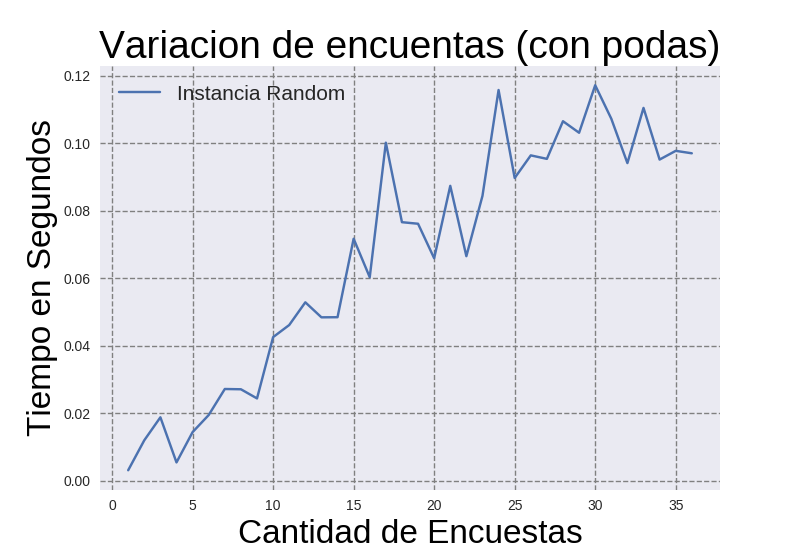
\includegraphics[scale=0.45]{VariacionesConPodas.png}
	\end{subfigure}
	\end{figure}
	
	Lo que podemos ver es que a medida que aumentamos el número de encuestas también aumenta el tiempo del algoritmo. Con lo que podemos concluir que la cantidad de encuestas afecta directamente al algoritmo. Esto se puede ver en la idea conceptual de árbol que ultilizamos antes, la idea sería que, a medida que crecen las encuestas, cuesta más pasar de un nivel a otro, ya que es ahi donde recorremos las encuestas para ver la confiabilidad de los agentes. 